%% LaTeX Beamer presentation template (requires beamer package)
%% see http://bitbucket.org/rivanvx/beamer/wiki/Home
%% idea contributed by H. Turgut Uyar
%% template based on a template by Till Tantau
%% this template is still evolving - it might differ in future releases!


% by:
% amir sohrabi

% this file is presented for assignment in scientific writing class 
% MEEN 653-600 Scientific Writing fall2014
% 

\documentclass{beamer}

\mode<presentation>
{
\usetheme{Warsaw}

\setbeamercovered{transparent}
}

\usepackage[english]{babel}
\usepackage[latin1]{inputenc}

% font definitions, try \usepackage{ae} instead of the following
% three lines if you don't like this look
\usepackage{mathptmx}
\usepackage[scaled=.90]{helvet}
\usepackage{courier}


\usepackage[T1]{fontenc}


\title{Introduction to \LaTeX}

\subtitle{A presentation for scinetific writing course}
% - Use the \inst{?} command only if the authors have different
%   affiliation.
%\author{F.~Author\inst{1} \and S.~Another\inst{2}}
\author{Amir Sohrabi\inst{1}}

\institute[Universities of]
{
\inst{1}%
Department of Mechanical Engineering\\
Texas A\&M University
}

\date{29 Sep 2014}


% This is only inserted into the PDF information catalog. Can be left
% out.
\subject{presentation for MEEN 653-600 Scientific Writing}

\AtBeginSubsection[]
{
  \begin{frame}<beamer>{Outline}
    \tableofcontents[currentsection,currentsubsection]
  \end{frame}
}


% If you wish to uncover everything in a step-wise fashion, uncomment
% the following command:

%\beamerdefaultoverlayspecification{<+->}

\begin{document}

\begin{frame}
  \titlepage
\end{frame}

	
\begin{frame}
\frametitle{Outline}
\tableofcontents
% You might wish to add the option [pausesections]
\end{frame}


\section{Introduction} 

\subsection{About \LaTeX  }
\begin{frame}{About \LaTeX \cite{LaTeX_wiki}}
\begin{itemize}
  \item \LaTeX was originally written in the early 1980s by Leslie Lamport at SRI
  \item It was releases in 1984
  \item \LaTeX is usually pronounced as: lay-tek or lah-tek
  \item Scientific written communication is done in \LaTeX
  \item It is good with displaying formulas
  \item Its can handle multiple language documents 
  \item It is distributed under a free software license 
\end{itemize}
\end{frame}

\subsection{Comparing Microsoft Word and \LaTeX}

\begin{frame} {Comparing Microsoft Word and \LaTeX}
\begin{itemize}
\item Word is not Free
\item It seems the there is no need to learn Word, \LaTeX has to be learned
\item In Word every thing is in the file, \LaTeX separates all the components 
\item Size of the files can be huge in Word, \LaTeX main file are normally smaller than 100KB
\item It takes up to minutes for Word to load, in \LaTeX file can be written in a note pad program
\item Word updates to new version that has problem with old files, \LaTeX is basically the same since begining with new features 
\end{itemize}
\end{frame}

\begin{frame} {Performance Test \cite{The_Beauty_of_LATEX}}
     \begin{columns}[t]
     \begin{column}[T]{5cm}
      Justification and hyphenation 
     \end{column}
     \begin{column}[T]{5cm} % alternative top-align that's better for graphics   
      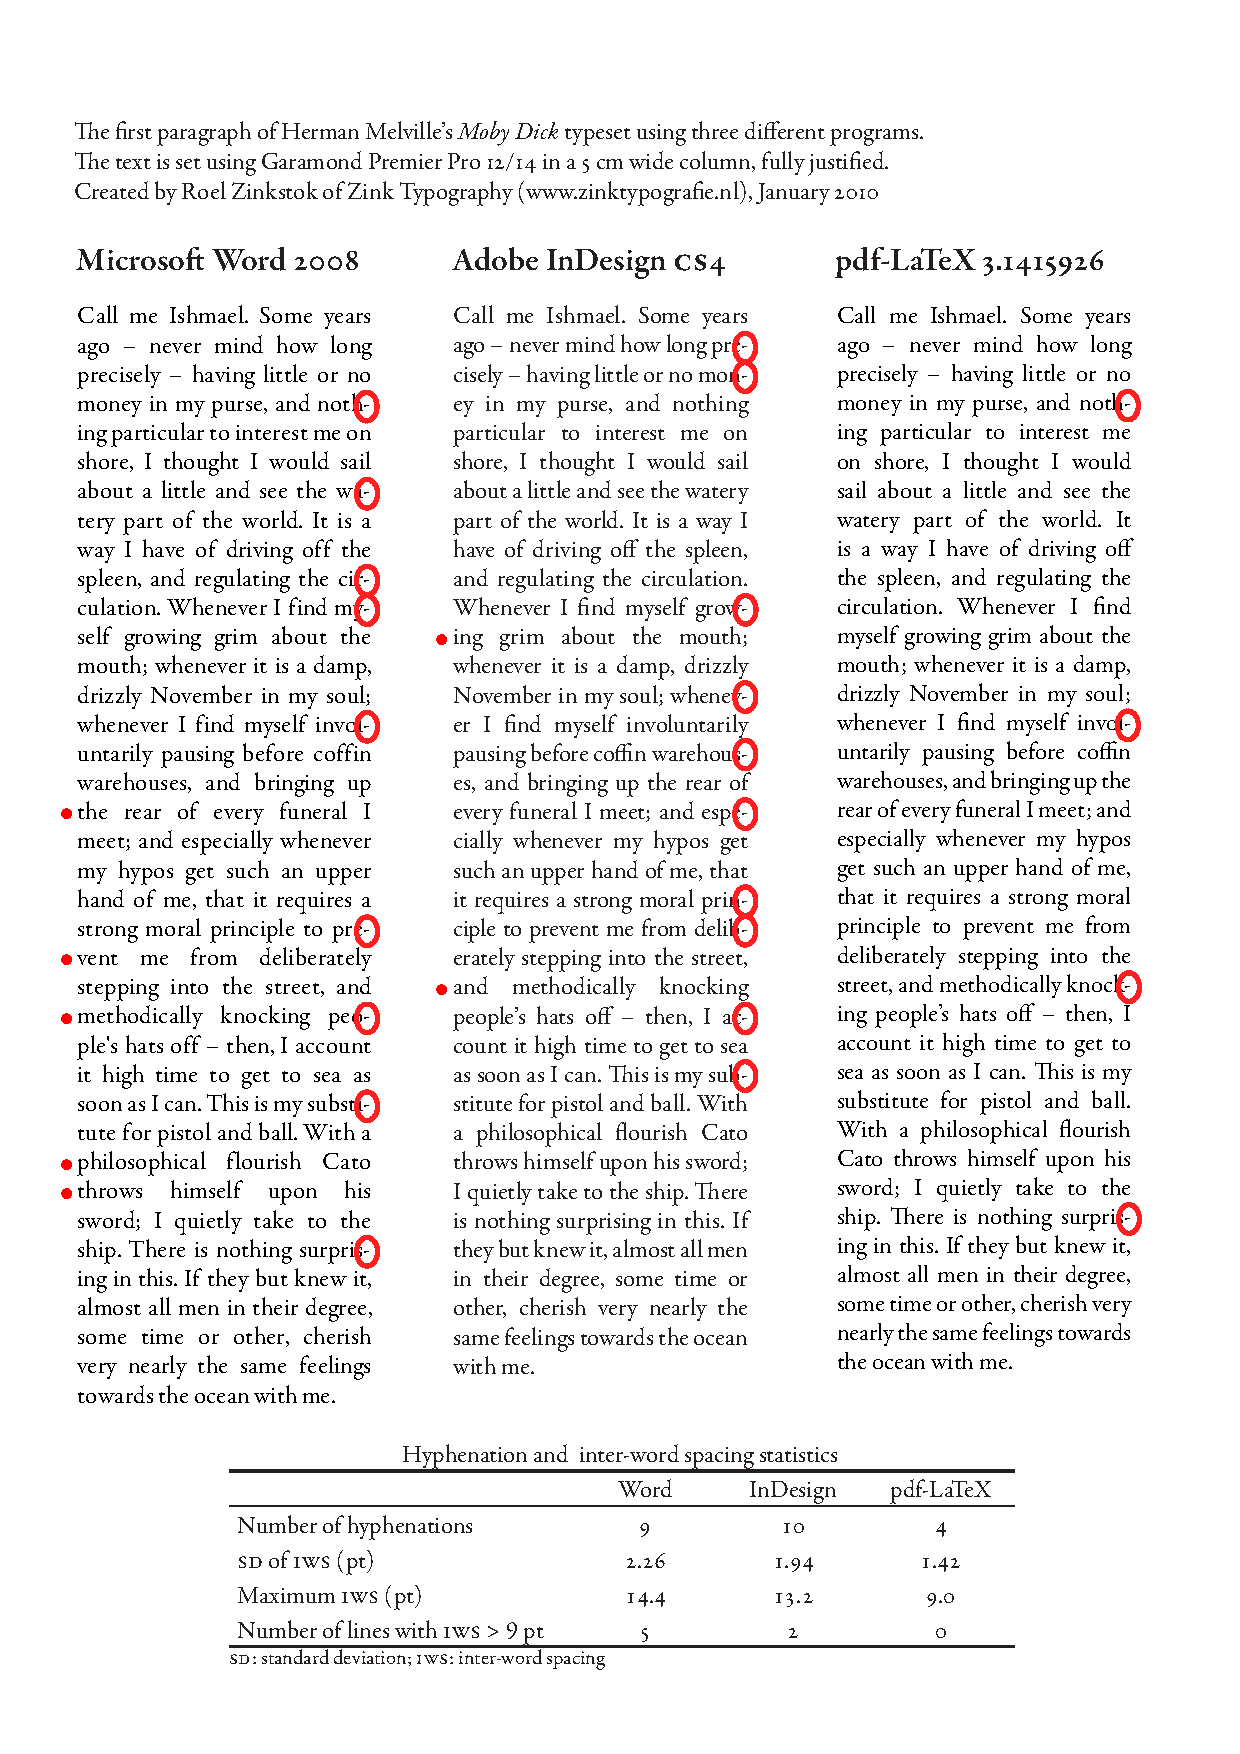
\includegraphics[height=5cm,trim = 0mm 0mm 00mm 0mm]{../figs/comparison.pdf}\\
     \end{column}
     \end{columns} 
\end{frame}


\section{Distibutions}

\begin{frame}{Distributions of \LaTeX}

     \begin{columns}[t]
     \begin{column}[T]{5cm}
      MiKTeX 
     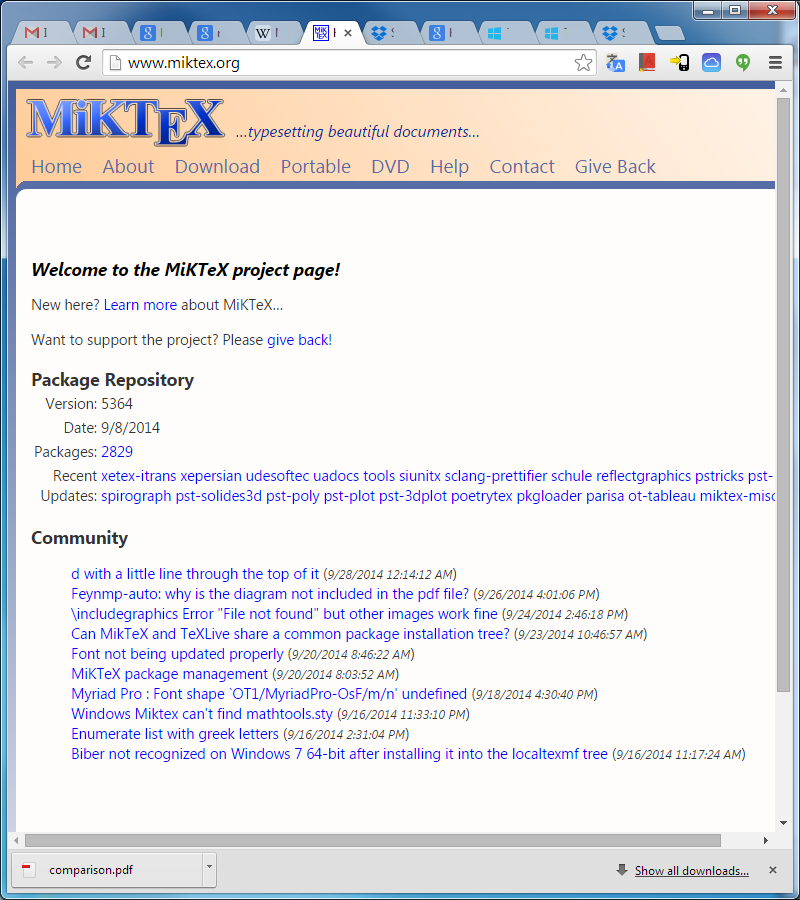
\includegraphics[scale=0.15,trim = 0mm 0mm 00mm 0mm]{../figs/MiKText.png}      
     \end{column}
     \begin{column}[T]{5cm} % alternative top-align that's better for graphics   
      TeXlive 
      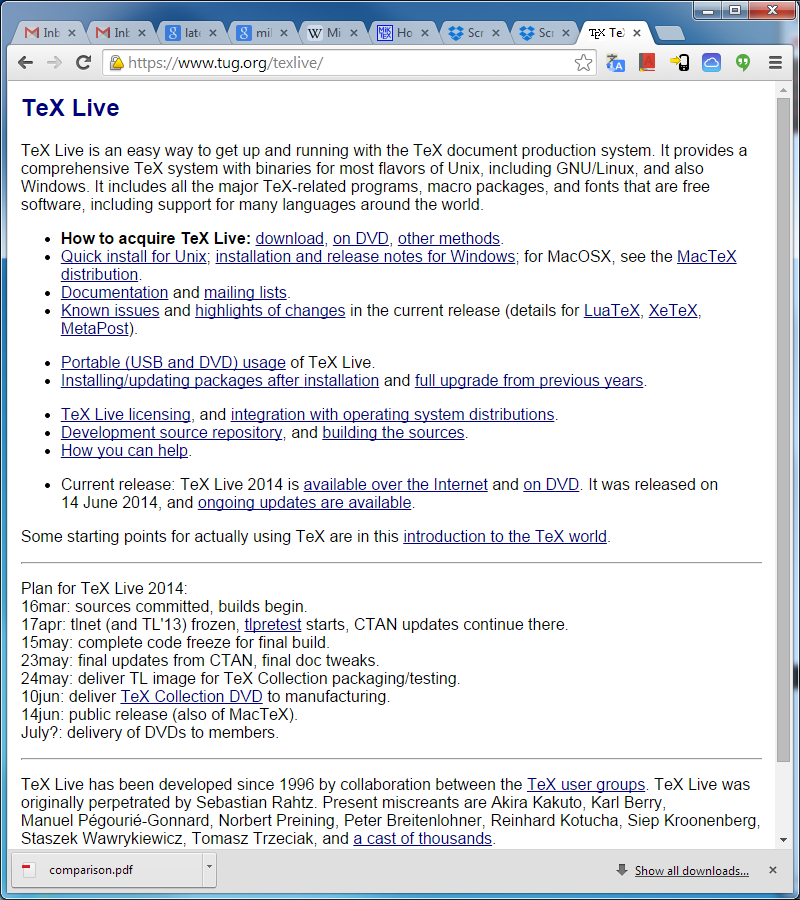
\includegraphics[scale=0.15,trim = 0mm 0mm 00mm 0mm]{../figs/TeXLive.png}         
     \end{column}
     \end{columns} 
         
\end{frame}


\section{\LaTeX editors}

\begin{frame}{\LaTeX  editors}
\centering
     \begin{columns}[t]
     \begin{column}[T]{3cm}
      \centering Texmaker 
      \begin{figure} 
     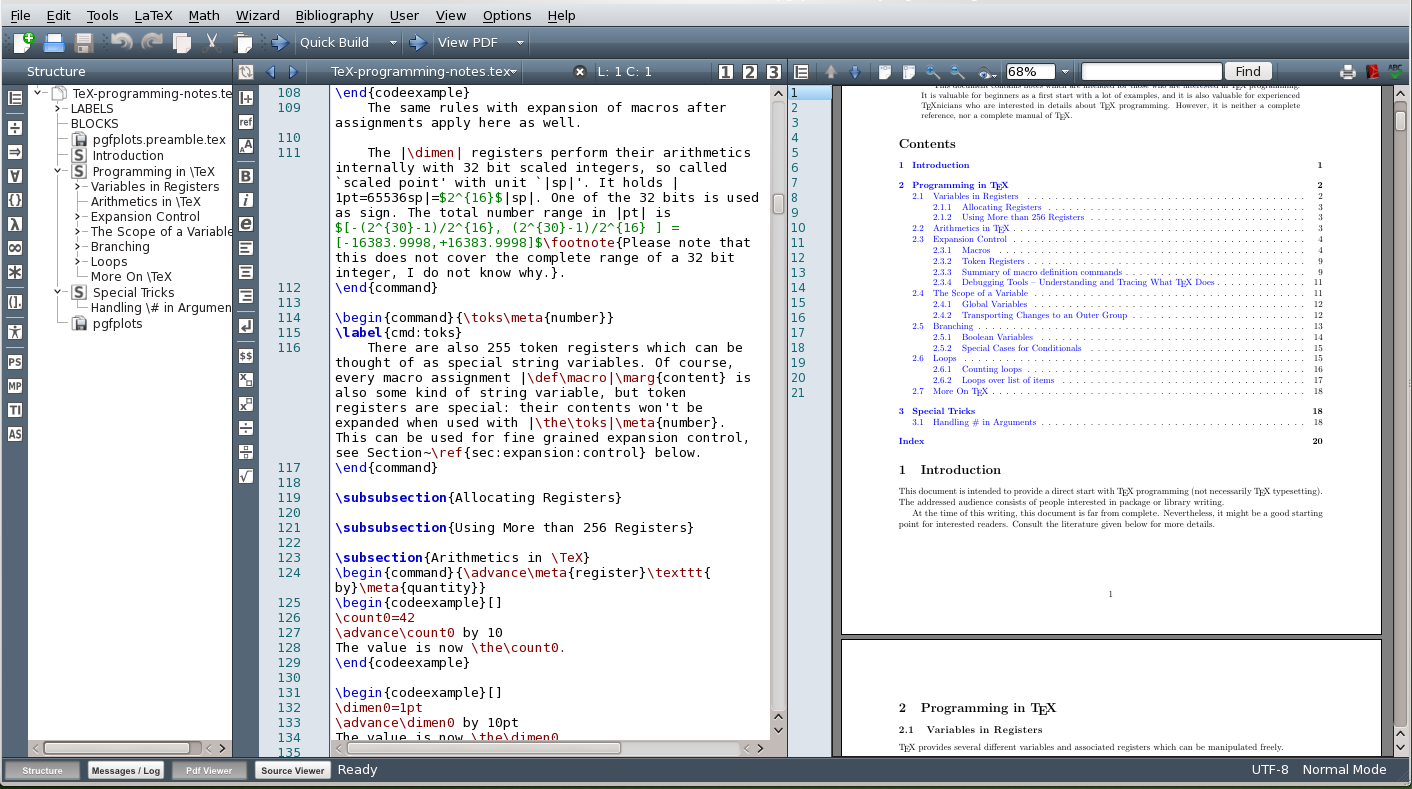
\includegraphics[height=2cm,trim = 0mm 0mm 00mm 0mm]{../figs/texmaker.png} 
     \end{figure}     
     \end{column}
     \begin{column}[T]{3cm} % alternative top-align that's better for graphics   
      \centering TeXworks
       \begin{figure}
     \includegraphics[height=2cm,trim = 0mm 0mm 00mm 0mm]{../figs/TeXworks.png}  
      \end{figure}       
     \end{column}
     \begin{column}[T]{3cm} % alternative top-align that's better for graphics   
      \centering TeXlipse 
      \begin{figure} 
      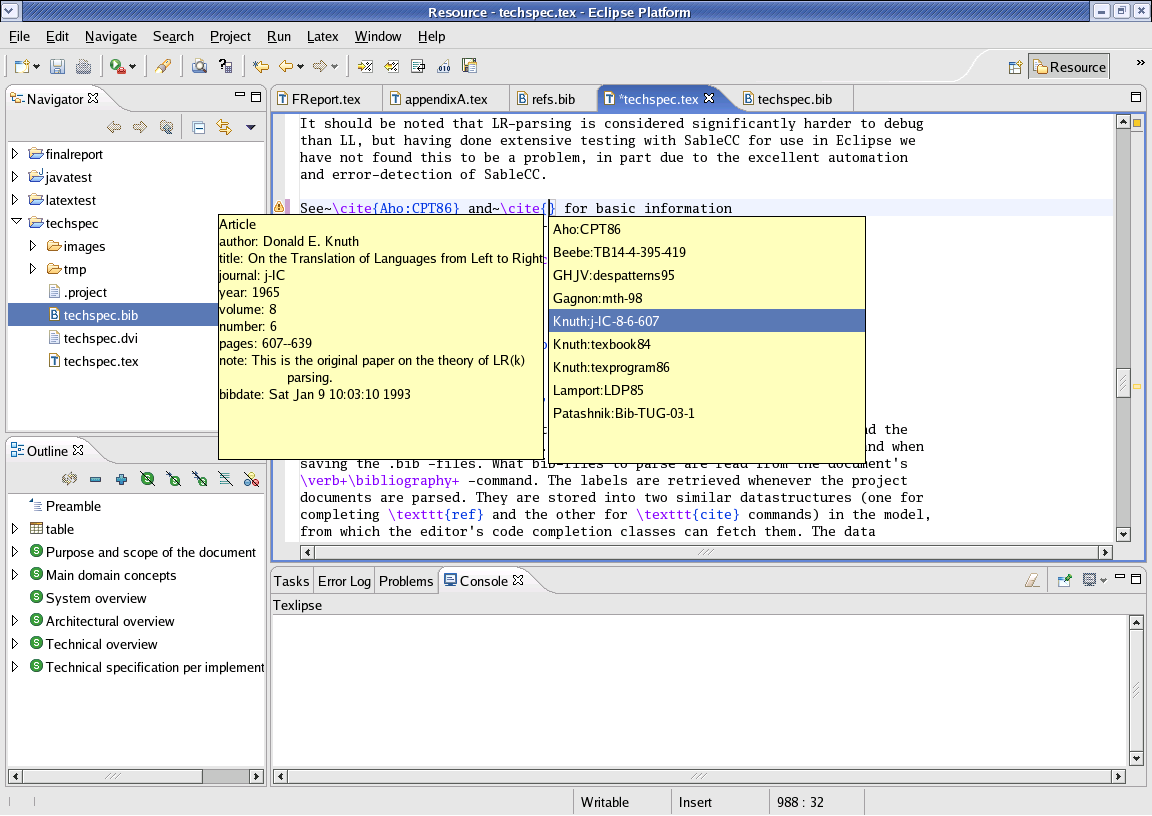
\includegraphics[height=2cm,trim = 0mm 20mm 0mm 0mm]{../figs/TexLipse.png}
      \end{figure}         
     \end{column}
     \end{columns} 
         
\end{frame}


\section{Structure of a document in \LaTeX}

\begin{frame}{Structure of a document in \LaTeX}
Different parts of the document
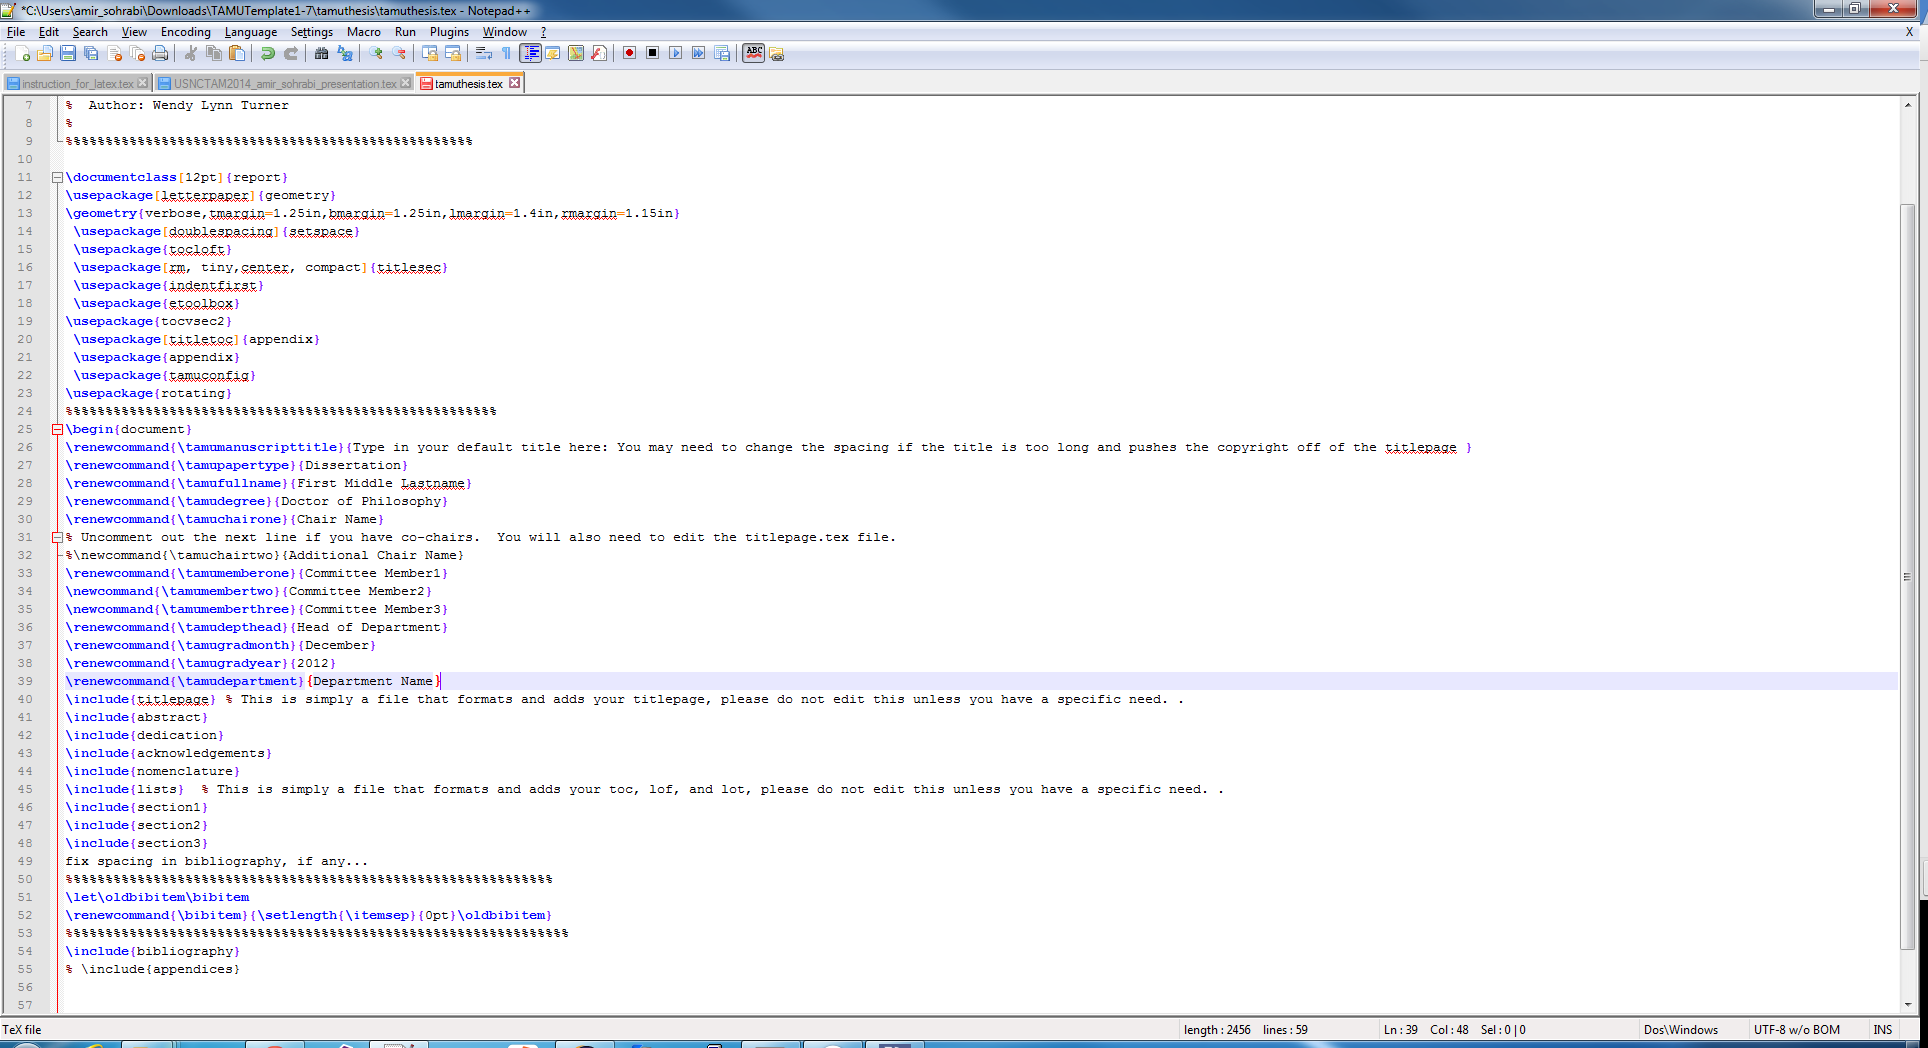
\includegraphics[height=6cm,trim = 0mm 20mm 0mm 0mm]{../figs/sample_thesis_document.png}
\end{frame}

\subsubsection{Usefull features of \LaTeX}
\subsubsection{Citation} 

\begin{frame}{Citation}

\begin{itemize}
  \item Citations are stored in a standard way
  \item They are printed and sorted as they are used and requested
  \item Numbering is automatic
  \item The style is defined already
  \item There are programs to manage the citations
  \item Citing directly from google scholar is possible 
\end{itemize}
\end{frame} 


\section{Writing in \LaTeX}
\begin{frame}{Writing in \LaTeX}  
\begin{itemize}
  \item Freedom in writing sentences
  \item Commenting the document is easier
  \item Reviewing will be faster
  \item Changing type of ducument is trivial
  \item Using version control is possible
\end{itemize}
\end{frame}

\begin{frame}[allowframebreaks]
\tiny
        \frametitle{References}
        \bibliographystyle{plain}
        \bibliography{references}
\end{frame}

\begin{frame}
\centering
Questions?
\end{frame}
\end{document}
